\chapter{Methods for Data Analysis} %8000
\label{ch:analysis}
Having looked at the kinds of questions that should be being asked, we will now turn to examine the methods that might be used to help answer those questions, and more importantly  to criticisms of those methods. In order to get the most out of these methods it is important that they are used within the limits of their applicability, the best way to assess this is by critical assessment of their use. There have been comparatively few quantitative spatio-temporal methods developed, when compared to purely temporal or spatial techniques. Of these, the vast majority are spatial methods.

\section{Spatial Analysis}
There are a variety of different ways of slicing up the large number of techniques for analysing spatial data, they will not all be catalogued here. The different theoretical schools of thought such methods are influenced by will only be roughly categorised. Modern approaches to Landscape analysis are often split into experiential/phenomenological or GIS based quantitative analysis \citep[491]{GravesMcEwan2012}. While there have been attempts to draw both schools of thought together, (e.g. \citealp{Lake:2007fk}) and even creating combined methods, such as \citet{Rennell2012}, \citet{Eve2012} and \citet{Millican2012}, this has not been hugely successful. 

With regard to criticisms of GIS based techniques, these are often either from a theoretical perspective, or a methodological perspective. With regard to the first category of criticisms, Llobera, an influential GIS practitioner, readily admits that when GIS is measured against Phenomenology's theoretical aims it falls short \citep[497]{Llobera2012}. Clearly this is not surprising and in fact ``this inferiority is rather a matter of opinion especially when compared against methods (if any) put forward within mainstream narratives'' \citep[498]{Llobera2012}. The theoretical elements of these criticisms are well rehearsed, focussing around dogmatic rejection of representations, particularly digital ones and have been addressed by \citet[498]{Llobera2012}. In fact Llobera concludes that the main criticisms in this vein are ``for the most part too generic or inconsistent to be constructive'' \citep[499]{Llobera2012}. \citet{eps364158} focuses on two key criticisms raised against visibility studies, firstly the objection that map like representations are specifically a modern, western construction, which we cannot assume is shared by other cultures \citep[118]{eps364158}. And secondly the suggestion that such studies privilege vision over other aspects of bodily engagement \citep[118]{eps364158}. With regard to the first, after considering early evidence of map creation and map like thinking from cultures as diverse (spatially and temporally) as ancient Peru and Babylonia Wheatley robustly disregards the criticism: ``There are good reasons, then, not to uncritically accept the assertion that non-western, non-modern cultures cannot or could not engage in this kind of spatial abstraction'' \citep[119]{eps364158}. However he does note, that this line of critique can be constructive, in forcing us to consider the culturally specific ways we currently use to represent space \citep[118]{eps364158}. With the second criticism, however,  Wheatley has some sympathy, he concludes that while there is evidence that vision may be naturally privileged by humans, we are not solely visual creatures \citep[121]{eps364158} and that ``a more interesting line of investigation would therefore lead to the development of methods for exploring how the senses may be related to one another in the structuring of space'' \citep[121]{eps364158}.

From some of the more nuanced criticism it is possible to discern methodological issues that must be considered when such analytical methods are employed, for example \citet{Llobera2012} identifies:
\begin{enumerate}
\item inadequacies with spatial methods to address the kind of questions asked by interpretive approaches
\item spatial representations are often abstracted, mismatched in terms of scale and precision from the questions asked
\item GIS often does not deal with space as it surrounds an individual
\end{enumerate}

To this can be added the recommendation from \citet{eps364158}, that there is clear potential in considering how the senses operate together to create an experience of place. Going further, there is clearly the opportunity to explore how this could translate into spatial patterning \citep[122]{eps364158}, modulated by spatial scale \citep[123]{eps364158}, which would ``offer the possibility of methodological application because they can be modelled and so are amenable to the development of robust, formal methods while they remain at the same time deeply relational and contextual'' \citep[124]{eps364158}.

Other specific, methodological issues, often raised by GIS practitioners themselves, are crucial when considering the specific analytical method, but have less impact on the wider issue of GIS based quantitative analysis. However, there have been wider criticisms raised, for example the notion of the theoretical neutrality of GIS has been considered indefensible since \citet{Wheatley:1993qf}. With this in mind, it is important that analytical techniques are not simply applied as mere tools, but that their theoretical underpinnings are understood. 

Apart from the correct application of appropriate methods, a key area of improvement would be the alignment of appropriate methods with questions. A complaint raised against many methods is that they are epistemologically limited and encourage the creation of an objectified, god's eye view \citep[512]{Rennell2012}, which is the source of the mismatch between our knowledge about the world, and our knowledge about the world as experienced \citep[498]{Llobera2012}, although \citet{eps364158} argues contrary to this, as discussed above. A part of this problem is that most spatial analysis often lacks any consideration of the temporal structure of space, as such geographical areas are represented in an idealised a-temporal way. For example, \citet{wheatley1995cumulative} presents all the sites as though outside of time, as there is no consideration of the sequencing of the construction of monuments, and therefore of the incremental changes to the visual structure of the landscape. By combining time and space into the same analysis it will be much easier to represent the world as it may be have been. And it may in fact add an extra dimension of being-in-the-world, by studying sites at particular points in time and in their history. 

Before delving into time, let us track back slightly, and consider the other main spatial approach, the experiential or phenomenological landscape approach. This is not without its critiques, although \citet[512]{Rennell2012} argues that many criticisms are still raised against older, more provocative pieces of phenomenological writings and lump these with progressive subject centred approaches, without considering their distinctions. A particularly important criticism is the lack of dialogue, especially from the experiential side of the argument \citep[601]{Gillings2012}, without which it is difficult to forge a unified approach to landscape analysis. In fact, Gillings goes on to suggest that the two approaches are intractable and that it would be more profitable for quantitative researchers to develop their own theoretical frameworks \citep[610]{Gillings2012}. Others have suggested techniques, such as scaffolding methods, should be used to bridge the gap between empirical information and narratives \citep{Llobera2012}. This difficulty in going from theory to method has been recognised (e.g. \citealp[500]{Llobera2012}) as more complicated for certain theories, such as phenomenological derived ones, with part of the problem being the lack of a defined body of theory, and the focus of such theories on ``complexity through detailed context-rich narratives'' \citep[503]{Llobera2012}. This clearly relates to the previous chapters examination of the questions that are asked, however as this project is approaching combined spatio-temporal analysis from the angle of spatialising time, a thorough analysis and appraisal of spatial questions and how phenomenological questions can be answered by GIS will be left for the future, perhaps, for a project to temporalise space.

In terms of phenomenological or subject-centred approaches to analysis, a critical concern from a temporal perspective, is that such analysis are based firmly in the present and pay little regard to the changes that will have taken place in the landscape over time. As such, it is really only possible to study modern people's relationships with a site, or landscape and infer back to the experiences of past people. But surely, to truly understand the experiences of people in the past it is essential to attempt to understand the landscape as it was, for people then and through the ages, how it has developed through time, including peoples relationship with their past through the landscape. Is it truly feasible, for a modern archaeologist to understand a past person's relationship with their past by simple experiencing a modern landscape? 

\section{Temporal Analysis}
There are few quantitative temporal analytical techniques, fewer still that are routinely applied to archaeological questions, with most studies taking a more narrative or descriptive approach (e.g. \citealp{Bradley:2002fk,Bailey:2007fk}). This is perhaps because it is hard to completely remove the spatial component. There has been some interest in aoristic based approaches, such as \citet{Crema2012} and \citet{Baxter2016120}, although most aoristic analysis has been spatio-temporal, so will be covered in section~\ref{sec:sta} below. The two most prominent forms of temporal analysis are bayesian modelling and summed probability distribution, both approaches operate (primarily) with radiocarbon dates, the merits and criticisms of both shall be considered in turn.

\subsection{Bayesian Modelling}
Probably the most frequently used quantitative temporal approach is the bayesian modelling of radiocarbon dates, which has increased in use dramatically from around 2006 onwards, \citep[679]{doi:10.1080/00438243.2015.1067640} and which forms a core part of large scale projects such as Gathering Time \citep{Whittle:2011kl,Whittle:2011tg} and the Times of Their Lives \citep{whittle2018times}. The claims for this approach are considerable, including being a third radiocarbon revolution \citep[126]{azu_rc3483}, and that it can in some cases produce chronologies with a resolution of decades \citep[141]{azu_rc3483} although, it should be noted that the approach is not limited to radiocarbon determinations \citep{Millard:2003fk}. However, as an approach it is not without issues, with several recent works taking a critical evaluation to the corpus of studies using bayesian methods to model dates\citep[e.g.][]{doi:10.1080/00438243.2015.1070082,doi:10.1080/00438243.2015.1053977,doi:10.1080/00438243.2015.1065759}. Some of the common themes of such criticisms include:

\subsubsection{Validity of the Model}
The validity of the model is one of the two main issues identified by \citet{doi:10.1080/00438243.2015.1070082}. Fundamentally it is about whether the archaeologist's interpretation of the chronology as represented in the model is valid. There are more detailed nuances, such as: whether the questions the archaeologist is trying to answer are amenable to modelling; if they will be answered by this model \citep[531]{doi:10.1080/00438243.2015.1070082}; and the archaeologist's skill in constructing models, for example whether the use of boundaries is valid \citep[533]{doi:10.1080/00438243.2015.1070082}. A robust example of this is presented in \citet{doi:10.1080/00438243.2015.1065759} when examining bayesian modelling of Palaeolithic dates. The issue is encountered in the first instance by assuming a Mousterian overlap with the Ch\^atelperronian, as evidenced by dating Mousterian sites outside of the Ch\^atelperronian's known distribution, and secondly by combining evidence for human and carnivore occupations in the same phase in the model \citep[603]{doi:10.1080/00438243.2015.1065759}. This issue can be thought of as ``the relationship between the dated event and the target event'' \citep[689]{doi:10.1080/00438243.2015.1067640} and it is important that the modeller is sure of the association between the two events, in particular they must be confident they can determine if a sample is residual or intrusive. While it may be impossible to guard against this issue entirely, as it is in part down to subjective interpretation, it is crucial that the modeller understands the implications of choices made when constructing the model. Further protection can in this case be provided by critical review and re-evaluation of published models \cite{doi:10.1080/00438243.2015.1070082}.

\subsubsection{Reliability of Prior Information}
Reliability of prior information is the second of the two main issues covered by \citet{doi:10.1080/00438243.2015.1070082}; it ultimately boils down to the reliability and applicability of the dated samples. In fact, they assert that ``the main responsibility of archaeological users of bayesian models is to ensure the reliability of the prior information upon which models are based'' \citep[527]{doi:10.1080/00438243.2015.1070082}. Clearly there is some overlap with the previous criticism, in particular with assessing residuality. There are some clear guidelines, which can be used to increase confidence in chosen priors, for example ``dated samples must reflect human activity'' \citep[532]{doi:10.1080/00438243.2015.1070082} and it is important to be confident in their stratigraphic location. It is also recommended that all priors be justified by the modeller \citep[537]{doi:10.1080/00438243.2015.1070082}. \citet{doi:10.1080/00438243.2015.1067640} recommends authors provide sufficient details of their priors, such that their reliability can be easily assessed by others. This would include: calculation details, references to laboratory methods, associated measurements \citep[687]{doi:10.1080/00438243.2015.1067640}, and ideally also other details such as carbon reservoir, age at death, single entity, etc \citep[690]{doi:10.1080/00438243.2015.1067640}. These are not mere technical details, for example, \citet[610]{doi:10.1080/00438243.2015.1065759} discuss the effect of dragging of modelled dates by the inclusion of older dates, which don't use modern pre-treatment methods. And it is perhaps for this reason that \citet{doi:10.1080/00438243.2015.1070082} recommend that samples should only be included in a model if they have been subject to robust pre-treatment methods, which are fully delineated \citep[537]{doi:10.1080/00438243.2015.1070082}.

\subsubsection{Small Numbers of Priors}
A small number of priors is a problem encountered by \citet[604]{doi:10.1080/00438243.2015.1065759}, where the limited number of dates in a model means it is highly sensitive to each individual prior. On a similar vein \citet{doi:10.1080/00438243.2015.1070082} pose the question ``another source of error is when single layers are represented by only one radiocarbon measurement. How do we know if this is accurate?'' \citep[530]{doi:10.1080/00438243.2015.1070082}. Related to this problem is that of selecting samples, as \citet{doi:10.1080/00438243.2015.1070082} notes, when samples are reviewed critically the pool of suitable samples diminishes. However this does not mean samples should be used un-critically, instead we must be wary of models which rely heavily on a small number of samples and where possible try to obtain more high quality samples.

\subsubsection{Uncritical Acceptance of Posterior Results}
The problem of uncritical acceptance of posterior results has been identified by \citet[528]{doi:10.1080/00438243.2015.1070082} and relates to the uncritical acceptance of posterior results from priors or models with one or more of the previous issues. This data is then fed into further analysis where it is accepted at face value. Surely, any inferences drawn from such a bayesian model should have the same, if not greater uncertainty than their constituent parts. In fact if we are suspicious of a prior value, why include it in a model in the first place? The result of this is a situation where the probability distribution is not necessarily representative of the actual probability; if there are samples with some doubt attached surely this should be modelled, so that the doubt is represented in the probability distribution, or dubious results should simply be discounted.

\subsubsection{Bayesian Analysis in Gathering Time}
The bayesian analysis of Gathering Time seeks to create an almost historical narrative of the early Neolithic \citep[800]{Whittle:2011tg}, with a particular focus on the enclosures of southern Britain. This is achieved by building up an increasingly abstracted view of dates from such enclosures. The process starts at the smallest level, each dated sample is listed and described, e.g. for Windmill Hill see \citet[68]{Whittle:2011kl}. These dates are then combined into a bayesian model of the chronology (e.g., \citealp[83]{Whittle:2011kl}) which for larger sites is done in sections with another more abstracted model created for the whole site e.g. \citealp[83]{Whittle:2011kl}. A key part of these models is the generation of so called boundary events: at the very least there will be a start and end for each site, depending on the extent of dating and specific research questions, often more. The boundary events for all the sites in a wider geographical area, such as the North Wiltshire Downs are used to build a model for that wider area, (e.g. \citealp[106]{Whittle:2011kl}) even larger areas, such as southern, or eastern England are then considered in the same way (e.g. \citealp[684]{Whittle:2011tg}). Finally, further models are derived, for the start of all southern British enclosures (e.g., \citealp[687]{Whittle:2011tg}) and derived data, such as the duration of use across all enclosures (e.g. \citealp[706]{Whittle:2011tg}). The authors also construct models for other types of data, such as long barrows, linear monuments, and pottery. The refined dates provided by the large number of bayesian models are then used to build up a narrative of the early British Neolithic \citep[800]{Whittle:2011tg}. Tying all the different elements together into a unified proto-history of where practices and material culture first appeared and the rate at which it spread over the country.

The process taken to build up these models (unsurprisingly) meets the criteria as set out by \citet{doi:10.1080/00438243.2015.1067640} covering the themes identified above as validity of the model and reliability of prior information. However, the themes of small numbers of priors and of uncritical acceptance of posterior results require further investigation. Of the 38 enclosures examined in the text (more are included, but have no dates), there is quite a range in the number of dates per site. The smallest number of dates for a site that are included in the models is one, Combe Hill, while the largest is Hambledon Hill with 162. In this case, Combe Hill is modelled differently to Hambledon (as a TAQ in \citealp[687]{Whittle:2011tg}). The site with the smallest number of dates that is included in the model as a first class entity (in the same way Hambledon is included, by boundary values) is Court Hill, which has two dates in its model. Figure~\ref{fig:date-counts} shows a histogram of the number of dates or samples used in the study, the line widths being five dates. It clearly shows that the vast majority (23) sites have fewer than ten dates, ten sites have between 20 and 33 dates, and one each has 43, 46, 62, 76 and 162 dates. 

\begin{figure}
\centering
	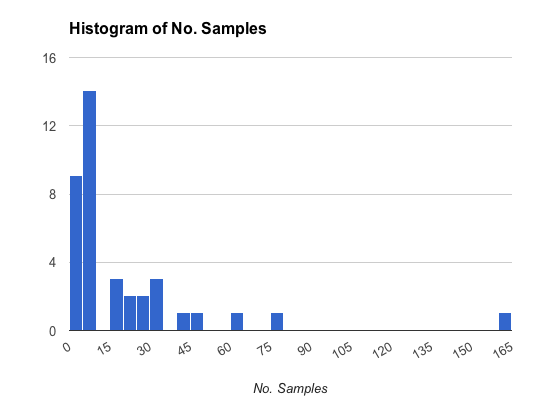
\includegraphics[width=0.6\textwidth]{figures/date-counts}
  \caption{Histogram of number of dated samples for sites included in Gathering Time}
  \label{fig:date-counts}
\end{figure}

Once these sites are abstracted away from their original models into boundary events they are (apart from Combe Hill) all represented in the same way, there is no indicator of the strength of evidence that lies behind these values. Such a metric could be taken as a measure of durability of the value, for example it is less likely the start and end dates calculated for Hambledon Hill will be refined by further fieldwork, but it is quite likely, even probable that more fieldwork would result in the values for Court Hill to be updated.

The abstraction of models into boundary events causes other problems. A clear example is Whitehawk Camp, where the limitations of the dating evidence are made clear in the text, for example the ``only dateable material from the primary chalk rubble in Ditch II is a residue sample from a single sherd, which could have been redeposited. The date of Ditch IV depends on non-optimal samples, and those for both Ditches III and IV may relate to cuts rather than to the original circuits.'' \citep[226]{Whittle:2011kl}. However this does not stop the abstracted boundary events to be included in other models, at which point they are taken to be as valid as any other value. As well as the formal uncertainty of the radiocarbon dates, there is also an informal uncertainty of the validity of the dates (and in other cases the model e.g. at Haddenham, \citealp[277]{Whittle:2011kl}) but which disappears once sites have been abstracted to boundary events. While the alteration of a few dates is unlikely to make a big difference to the macro scale result, it might have been worth the authors exploring how much influence they had on the result, by running it again without boundary dates from sites with dubious dating evidence. More problematic would be an issue with a large number of sites.

The large number of sites with very few dates also points at a further potential problem, that of the limited spatial extent of archaeological investigations. For example at Court Hill, the area excavated was around 5m of ditch, out of around 175m \citep[242]{Whittle:2011kl} that is roughly 2.9\%. How confident are they that the reported dates accurately represent the start of activity at Court Hill? It is quite possible the site was dug over a period of time, as a succession of ditch segments, until it was completed and then underwent subsequent further use. Clearly, this is a problem with sites that have only undergone small archaeological investigations, with ultimately the only solution being to commission a full research programme on these sites. But this problem is not only limited to sites with a handful of dates, for example at Windmill Hill the inner ditch dates come from only four sections of ditch, the outer ditch dates come from only five sections, with less than 10\% of it having been excavated \citep[63]{Whittle:2011kl}. It is from this paucity of dated ditches that the inner-outer-middle order of construction is derived (which is in fact only 59\% probable \citealp[91]{Whittle:2011kl}) and it does not take into account the duration of the construction, only of use. In this model, each circuit is fully constructed before the next one is begun \citep[91]{Whittle:2011kl}. To a greater or lesser extent, this is a problem with all the enclosures examined in Gathering Time, caused in part by varying degrees of excavation, and also by the difficulty in finding suitable samples to date, especially in archived material. While total excavation might be ideal from the point of view of obtaining all possible data, it leaves nothing for future generations and is also extremely unlikely due to the cost and time it would take. A much more feasible approach is to make sure that excavated areas are relatively evenly distributed around the enclosure, as at Northborough \citep[328]{Whittle:2011kl} or Bury Hill \citep[240]{Whittle:2011kl} rather than The Trundle where all excavation is concentrated in one small area \citep[233]{Whittle:2011kl}. A not insignificant issue in Gathering Time is the difficulty of working out what the extent of excavated area is and from where around the enclosure circuit the dates have come from. For a start not every site has a plan, e.g. Maiden Bower \citep[265]{Whittle:2011kl} and those that do are of varying format and quality.

The lack of spatiality also extends to the larger scale analysis, for example, the analysis of Hambledon Hill within Cranborne Chase \citep[151]{Whittle:2011kl} lacks any plan and each regional analysis has only one large scale plan. The regional discussions do not provide maps that are more detailed or plans to illustrate the discussion and in fact hardly consider the spatial relationships and characteristics of the sites. There is also no attempt to match the humanising of time (through lifespans) with a humanising of space (by distance in travel times).

In summary, when done well the results from applying bayesian modelling to dates can be powerful, but unfortunately, it is not always done well. In an effort to improve quality, several authors have published best practices, for example \citet{doi:10.1080/00438243.2015.1067640}. However, it is clearly important that bayesian results are critically evaluated, and not simply accepted at face value. 

\subsection{Summed Radiocarbon Distributions}
Summed radiocarbon dates have been used as a method for determining the duration of archaeological phases \citep[9]{CAJ:676108} however when compared to bayesian methods they were found to create erroneously long estimates for durations of activity \citep[10]{CAJ:676108}. The problem is due to an implicit assumption that all the uncertainties are independent \citep[11]{CAJ:676108}. However the method is still used, a recent example of such an approach is demonstrated in \citet{AQY:9508563}, which compares summed radiocarbon probabilities across cultures, and bases its analysis on the assumption of random sampling \citep[1079]{AQY:9508563} contra \citet{CAJ:676108}. 

Summed radiocarbon dates have also been used contentiously as a proxy for population, with bold claims being made on the back of such analysis. A recent example of which is \citet{Shennan:2013fk} claiming patterns of population boom and bust in Neolithic Europe, and \citet{Collard2010866} using the method to show ``the Neolithic transition in Britain was mediated by a large influx of farmers from continental Europe''  \citep[869]{Collard2010866}. There has been a considerable amount of work undertaken to perfect the technique, for example correcting for statistical artefacts introduced by the calibration process, or for taphonomic loss such as by \citet{Williams2012578}. The methods used in such studies have become increasingly complex, for example \citet{Shennan:2013fk} take a null hypothesis approach, comparing their data set to the results from data generated by a model that exponentially increases the summed probability distribution through time. They then used a range of statistical significance tests to reject this null hypothesis and prove their conjecture - that there is a relationship between summed radiocarbon distributions and population density. 

There have been fundamental criticisms and corresponding defences of this approach, especially \citet{Torfing2015193,Timpson2015199,Torfing2015203}. Ultimately, according to \citet{Torfing2015203} the problems fall into two main areas, firstly he enumerates a set of assumptions that are required for the original assumptions of \citet{10.2307/281060} (on which the method is based) to be valid, these are:
\begin{enumerate}
\item People leave a comparable amount of material
\item All material is deposited in a similar manner that allow for equal preservation
\item Sites from all periods are equally excavated and dated
\end{enumerate}

Secondly, he analyses the use of sampling, as radiocarbon dates are often treated as a random sample. Torfing demonstrates that the ``radiocarbon date is only the last sample of a series of samples'' \citep[205]{Torfing2015203}. He goes on to argue that the link between population and radiocarbon dates is yet to be demonstrated, the lack of which could be particularly problematic if periods with different processes of site formation and preservation are compared. This criticism is effectively along the same vein as that made by \citet{CAJ:676108} about the nature of radiocarbon dates as samples. Three specific issues are analysed in \citet{Torfing2015193} as a criticism of \citet{Shennan:2013fk} and he concludes that the proposed model linking summed radiocarbon distributions and population is fundamentally flawed, ``several problems are still present: changes in monumentality, subsistence strategy and modern research foci are all systematic sources of error'' \citep[197]{Torfing2015193}.

These issues are summed up by a single succinct question, ``how does our proposed data-set relate to the questions we wish to answer?'' \citep[204]{Torfing2015203} and whereas he approaches the issues with a contextual analysis of the data, he is critical of proponents of summed probability distribution, as they ``mostly try to overcome these issues at the final step, that of the 14C-dates, and do not consider the formation of the record in the first place. The relevant problems lie outside the immediate calculations of the statistics, and are of a more fundamental character of how to use dates as data'' \citep[204]{Torfing2015203}. Specifically he is critical of the ``notion that if a large enough sample is used, and it is carefully treated with statistical tests, these sources of error will be insignificant'' \citep[193]{Torfing2015193} and argues that the quantities of datable material left by different activities are not necessarily comparable. Finally, he notes that any differences will persist in the archaeological record regardless of sample size \citep[193]{Torfing2015193}. 

In response to this criticisms \citet{Timpson2015199} respond with a mix of argument and hyperbole, including ``his subjective criticisms, lacking in any formal hypothesis testing, only serve to stagnate the discipline'' \citep[200]{Timpson2015199} and by claiming his lack of understanding of the method. They claim to be using proxies to only be showing correlation, however as \citet{Torfing2015203} points out this would only be valid if a relationship had already been proved between summed radiocarbon probabilities and population \citep[204]{Torfing2015203}. They also accuse him of not performing significance tests on his models, which is necessary due to the increase in sampling error caused by his use of specific (non random) subsets of the data \citep{Timpson2015199}. It would seem quite ironic that the proponents of a method that has been criticised for being reliant on assumptions of sample independence object to non-random sampling.

Summed radiocarbon distributions have also been used to analyse the changing importance of cereal cultivation through time by \citet{Stevens:2012fk, doi:10.1080/00438243.2015.1087330}. As with other approaches to summed radiocarbon distributions this method has not been without criticisms, \citet{doi:10.1080/00438243.2015.1072477,doi:10.1080/00438243.2015.1093427} concluded that the sample size was too small, that the results were in fact likely more to do with sampling strategy and that archaeobotanical evidence was capable of providing a much higher resolution picture of the use of cereal crops \citep[848]{doi:10.1080/00438243.2015.1072477}. 

Finally, there is a clear lack of a concern for the spatial in such studies. Taking a sample of five relatively recent studies, which are well regarded among proponents of the method, clearly demonstrates this lack. Across \citet{Shennan2013,TIMPSON2014549,10.1371/journal.pone.0105730,Shennan:2013fk,HINZ20123331} there is an average of less than one map or plan per publication and a variety of approaches for considering spatiality. \citet{Shennan2013} considers results only at the continental scale and a single region therein, where as \citet{HINZ20123331} considers 12 regions, examined in groups by the shape of results and then by comparisons across regions. Other publications sit somewhere along the spectrum from effectively a-spatial discussion to splitting an area up into a set of regions, which are examined independently. None perform any spatial analysis, or attempt to examine how population may be just as much a function of space as time, instead they simply accept the spatial variation and examine different regions separately.

The range of uses to which summed radiocarbon dates have been put suggest a fascination with them, but it is as though researchers see the distribution and think frequency, rather than probability. However, the same kinds of questions have been approached using alternative techniques, such as \citet{Steele20102017,BocquetAppel2009807}, which use a range of techniques for performing analysis on radiocarbon dates. It is to these other methods we should be turning and attempting to find ways to refine our highest quality data (such as through bayesian modelling) rather than dredging though large data sets hoping to find unproven correlations. While the summing of radiocarbon dates is primarily a temporal approach, the questions that are being asked, about the spread of Neolithic culture are fundamentally spatio-temporal in nature. Surely such questions are best answered by combined techniques, such as those that follow.

\section{Spatio-temporal Analysis} \label{sec:sta}
The number of attempted spatio-temporal analytical methods is relatively small, with some coming from research into Temporal-GIS, (hereafter T-GIS) and others as stand-alone pieces of research. The discussion of such software more generally will be deferred until the next chapter, the focus here will be on the spatio-temporal analysis performed using such systems.

One of the earliest attempts at spatio-temporal analysis (which has already been covered) was an extension of a spatial method, using the absolute date value as a property, for understanding the classic lowland Maya collapse. But it is necessary to turn to a different source to understand more recent spatio-temporal work. Johnson has had an impact as the source of multiple spatio-temporal methods, both from research into T-GIS and spatio-temporal analysis independent of such software. He was the first to build a T-GIS designed for archaeology, \citep{Johnson:1999cr, Johnson:2002kx} and also introduced aoristic analysis into archaeology \citep{Johnson:2004fk}, which has influenced a whole research tradition, e.g. \citet{Crema20101118}. 
While Johnson may have been one of the pioneers of T-GIS within archaeology, his resultant project, TimeMap does not seem to have been used for any archaeological study. Instead it has been limited to projects in the historical era, as its temporal model is unable to cope with probabilistic dates. So, in terms of spatio-temporal analytical methods TimeMap must be discounted, as it does not actually perform any that are of archaeological interest. Following on from Johnson, several authors have attempted T-GIS type systems with varying degrees of success, but few have attempted much in the way of spatio-temporal analysis. Most have simply described potential systems (e.g. \citealp{lock2002analysing}), or implemented mechanisms for storage and representation of the data. The exception to this being \citet{Green:2008fk} who implemented a T-GIS, which was then used as a platform for further analysis.

Green's analysis is mostly based around visual inspection (e.g. \citealp[156]{Green:2008fk}) of plots of radiocarbon dates. The dates are grouped by thematic layers, such as by period, these periods are then analysed sequentially, so that the result is a series of analysis of different time-slices. Crucially however, the background layer is not changed for each new time-slice and so is, in effect, static over time, for an example of this see figure~\ref{fig:green1}. The point plots for radiocarbon dates change, but the background is a map of all archaeological features from the site. This is quite problematic, as there is a logical disconnection between the dates and the archaeological features. It would make visual analysis and interpretation much easier, and more potent, if the features were associated with dates, then the combined two could be hidden or displayed for each plot. Another key problem with this is the arbitrary nature of the time slices, based on interpretative periods, as compared to other studies, which take the approach of taking time slices at regular intervals. There are problems with both approaches, for example, \citet{Crema20101118} notes that an approach with regular intervals can highlight changes within arbitrary periods. Conversely, if there is low temporal resolution between regular intervals it can appear as though there is little to no change between these intervals, but this is in fact an artefact of the data \citep[1121]{Crema20101118}. Clearly, neither approach is obviously a much better choice, this being the case we might reasonably expect an appraisal of the shortfalls of the chosen approach, but Green has not done this. 

\begin{figure}
\centering
	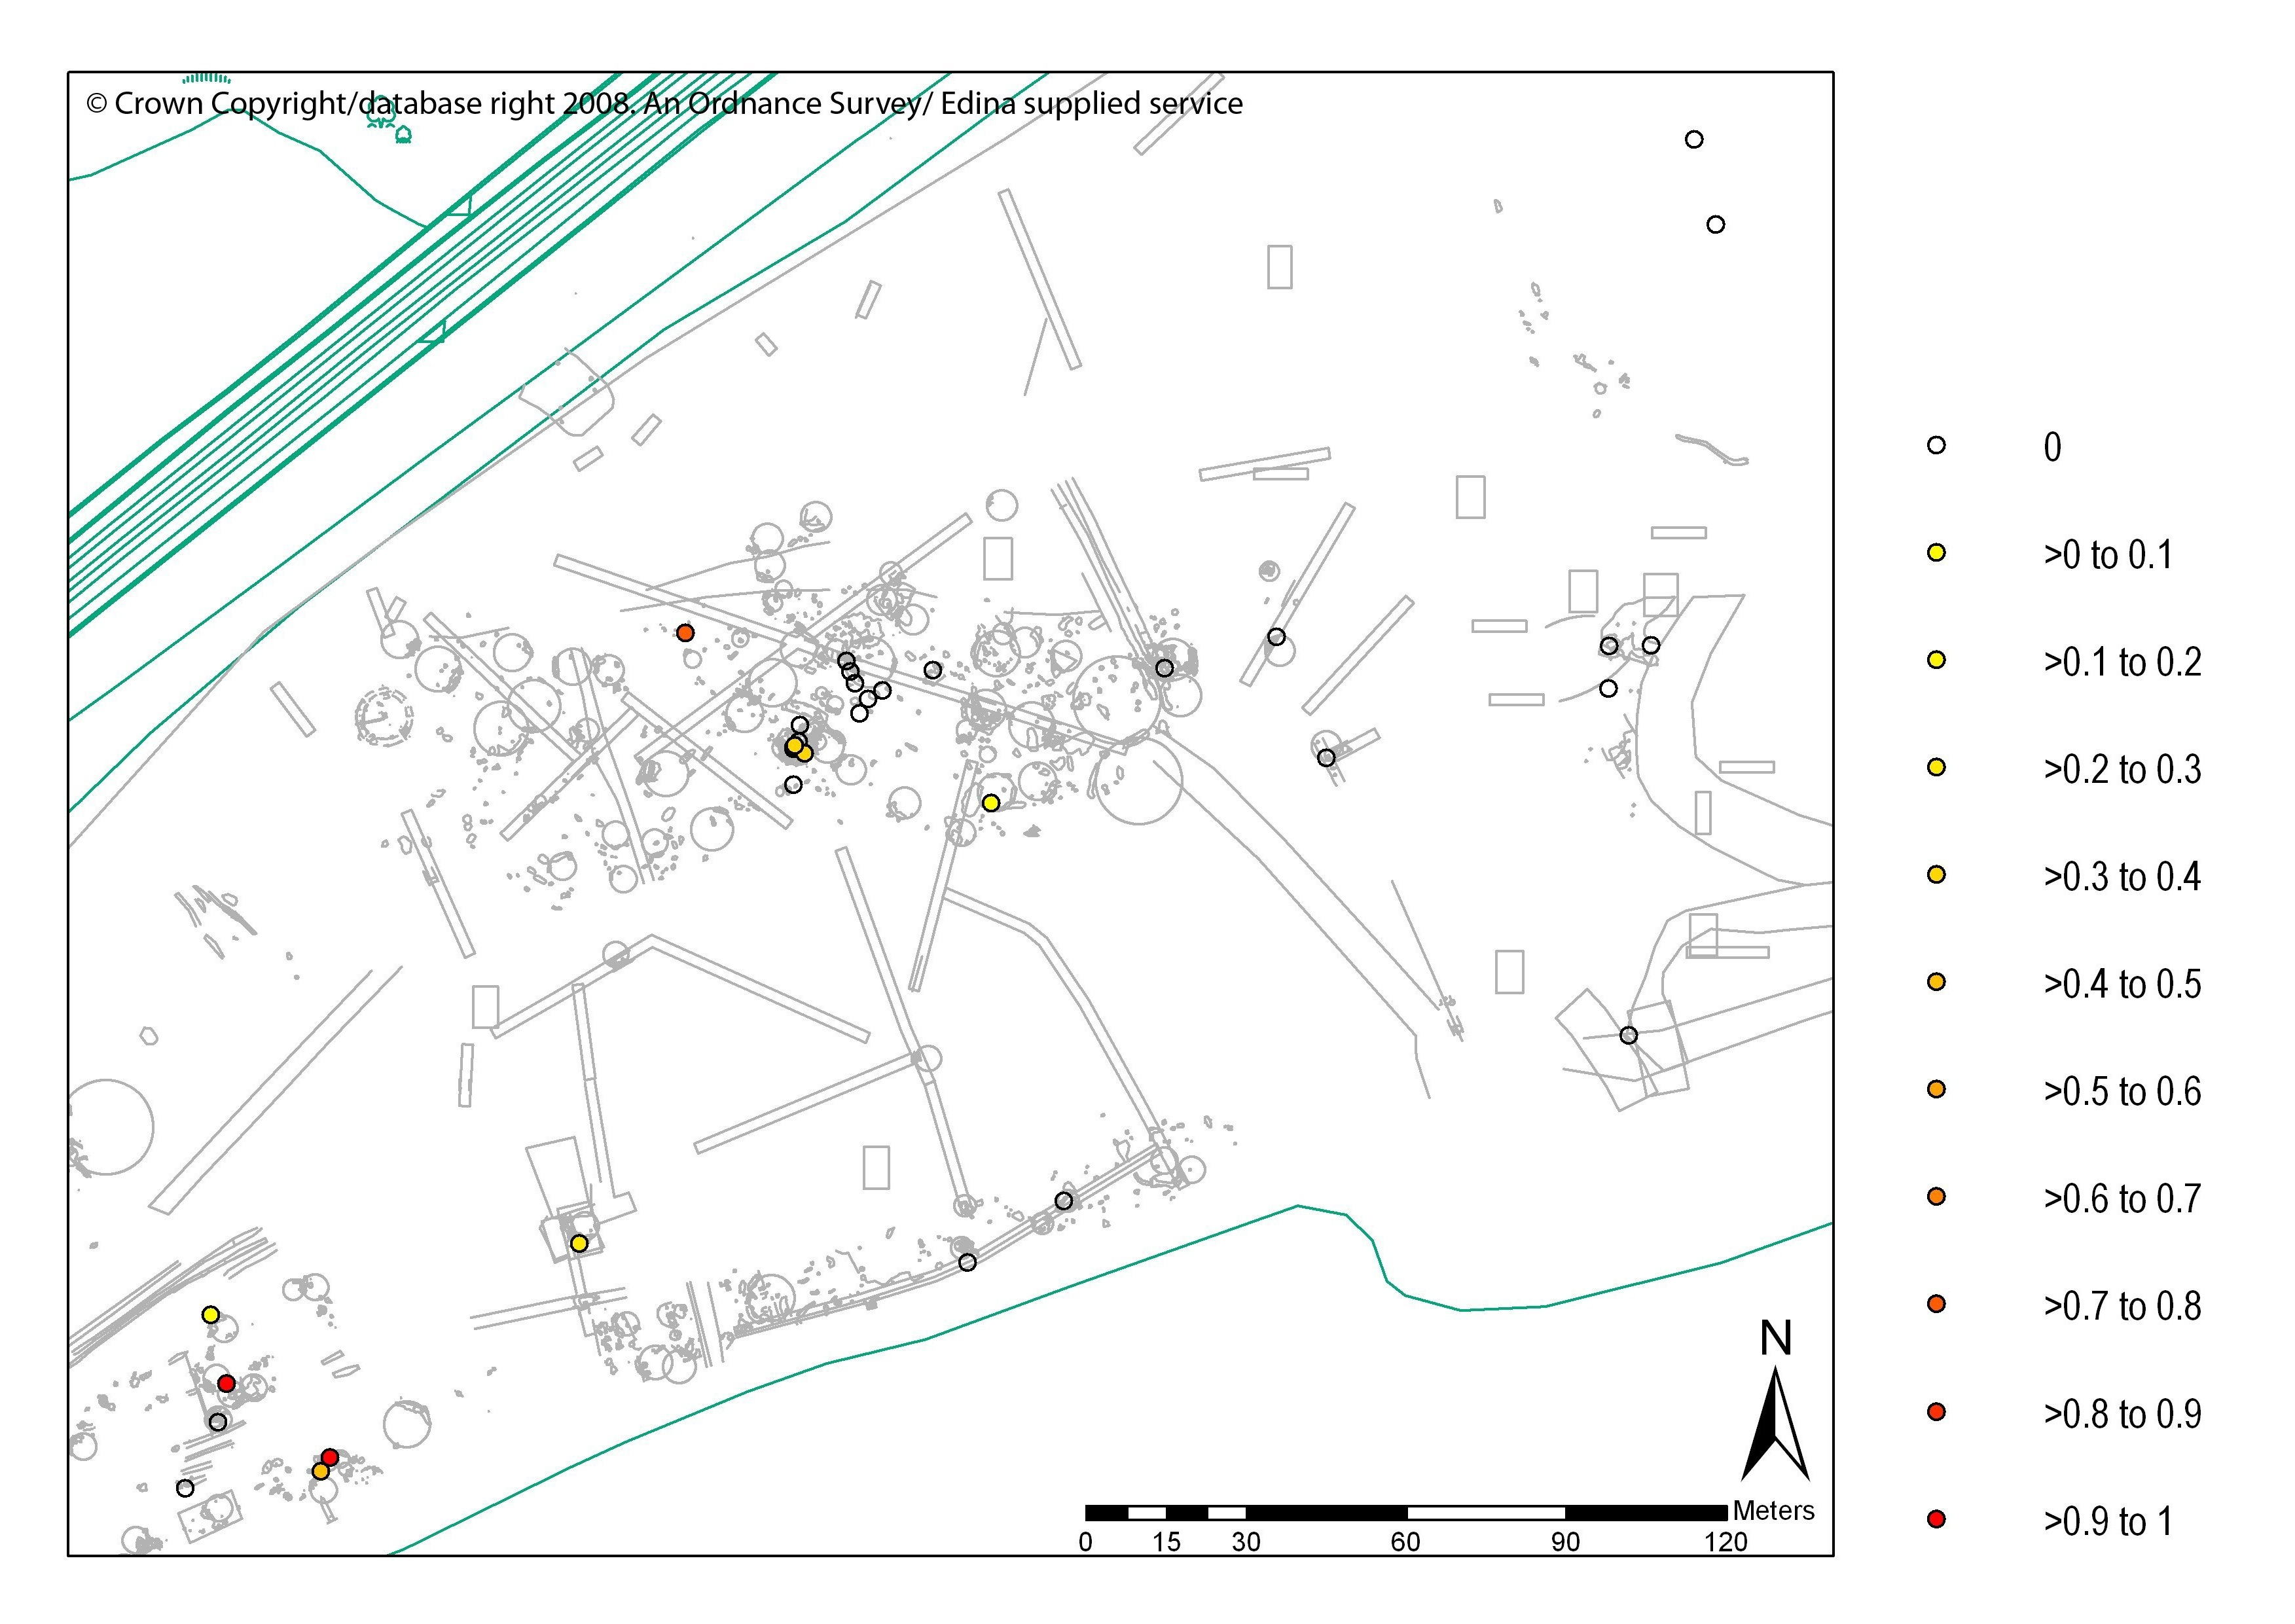
\includegraphics[width=0.9\textwidth,height=0.9\textheight,keepaspectratio=true]{figures/green1}
  \caption{Spatial distribution of un-modelled radiocarbon dates, coloured according to
probability of them falling within the period 4000-3500 cal BC, from \cite{Green:2008fk}}
  \label{fig:green1}
\end{figure}

In addition to this, Green also demonstrates the potential for spatio-temporal interpolation using his T-GIS, despite earlier in his thesis stating ``interpolation from time slices may be justified for evolutionary geographical change, but cannot capture the more random nature of cultural or historical change'' \citep[96]{Green:2008fk}, and that ``temporal interpolation of archaeology is complex and very uncertain. It is perhaps an act best left to the imagination, as computerised interpolation can give false authority to very speculative models'' \citep[98]{Green:2008fk}, and finally ``I do not believe that interpolation is the right way to approach temporal gaps in archaeological data: presenting a false completeness regarding our knowledge of the past has too great a potential to mislead.'' \citep[101]{Green:2008fk}. For two case studies Green makes use of interpolation, at an intra-site level these results ``give an indication of the probability of dates falling within any area of the site'' \citep[189]{Green:2008fk}. The analysis is performed on a per-period basis, demonstrating which areas have higher, and which have lower probabilities for a specified period. This is effectively being used as a proxy for use or activity of the site during each particular period. Of course, there are other potential reasons for lack of dates from certain areas, it may be a lack of use, it may also be down to a lack of datable material, or changing conditions. With only 65 radiocarbon determinations \citep[129]{Green:2008fk} spread across eight periods \citep[189]{Green:2008fk} they are likely to be highly influenced by any factors effecting recovery or applicability of radiocarbon methods. The validity of the interpolation then hinges on the validity of the quantity of radiocarbon dates for determining the relative past use, and of this Green does not provide evidence, especially for such a small sample size. Finally, by applying the interpolation without respect to the underlying archaeological features, the approximation of use created by the interpolation might actually be less accurate than a thorough examination of the archaeology. Specifically, it will smooth through dramatic changes in values, for example between successive indoor and outdoor spaces. See figure~\ref{fig:green2} for an example interpolation from Green's first case study, showing the interpolation overlaying features from all periods.

\begin{figure}
\centering
	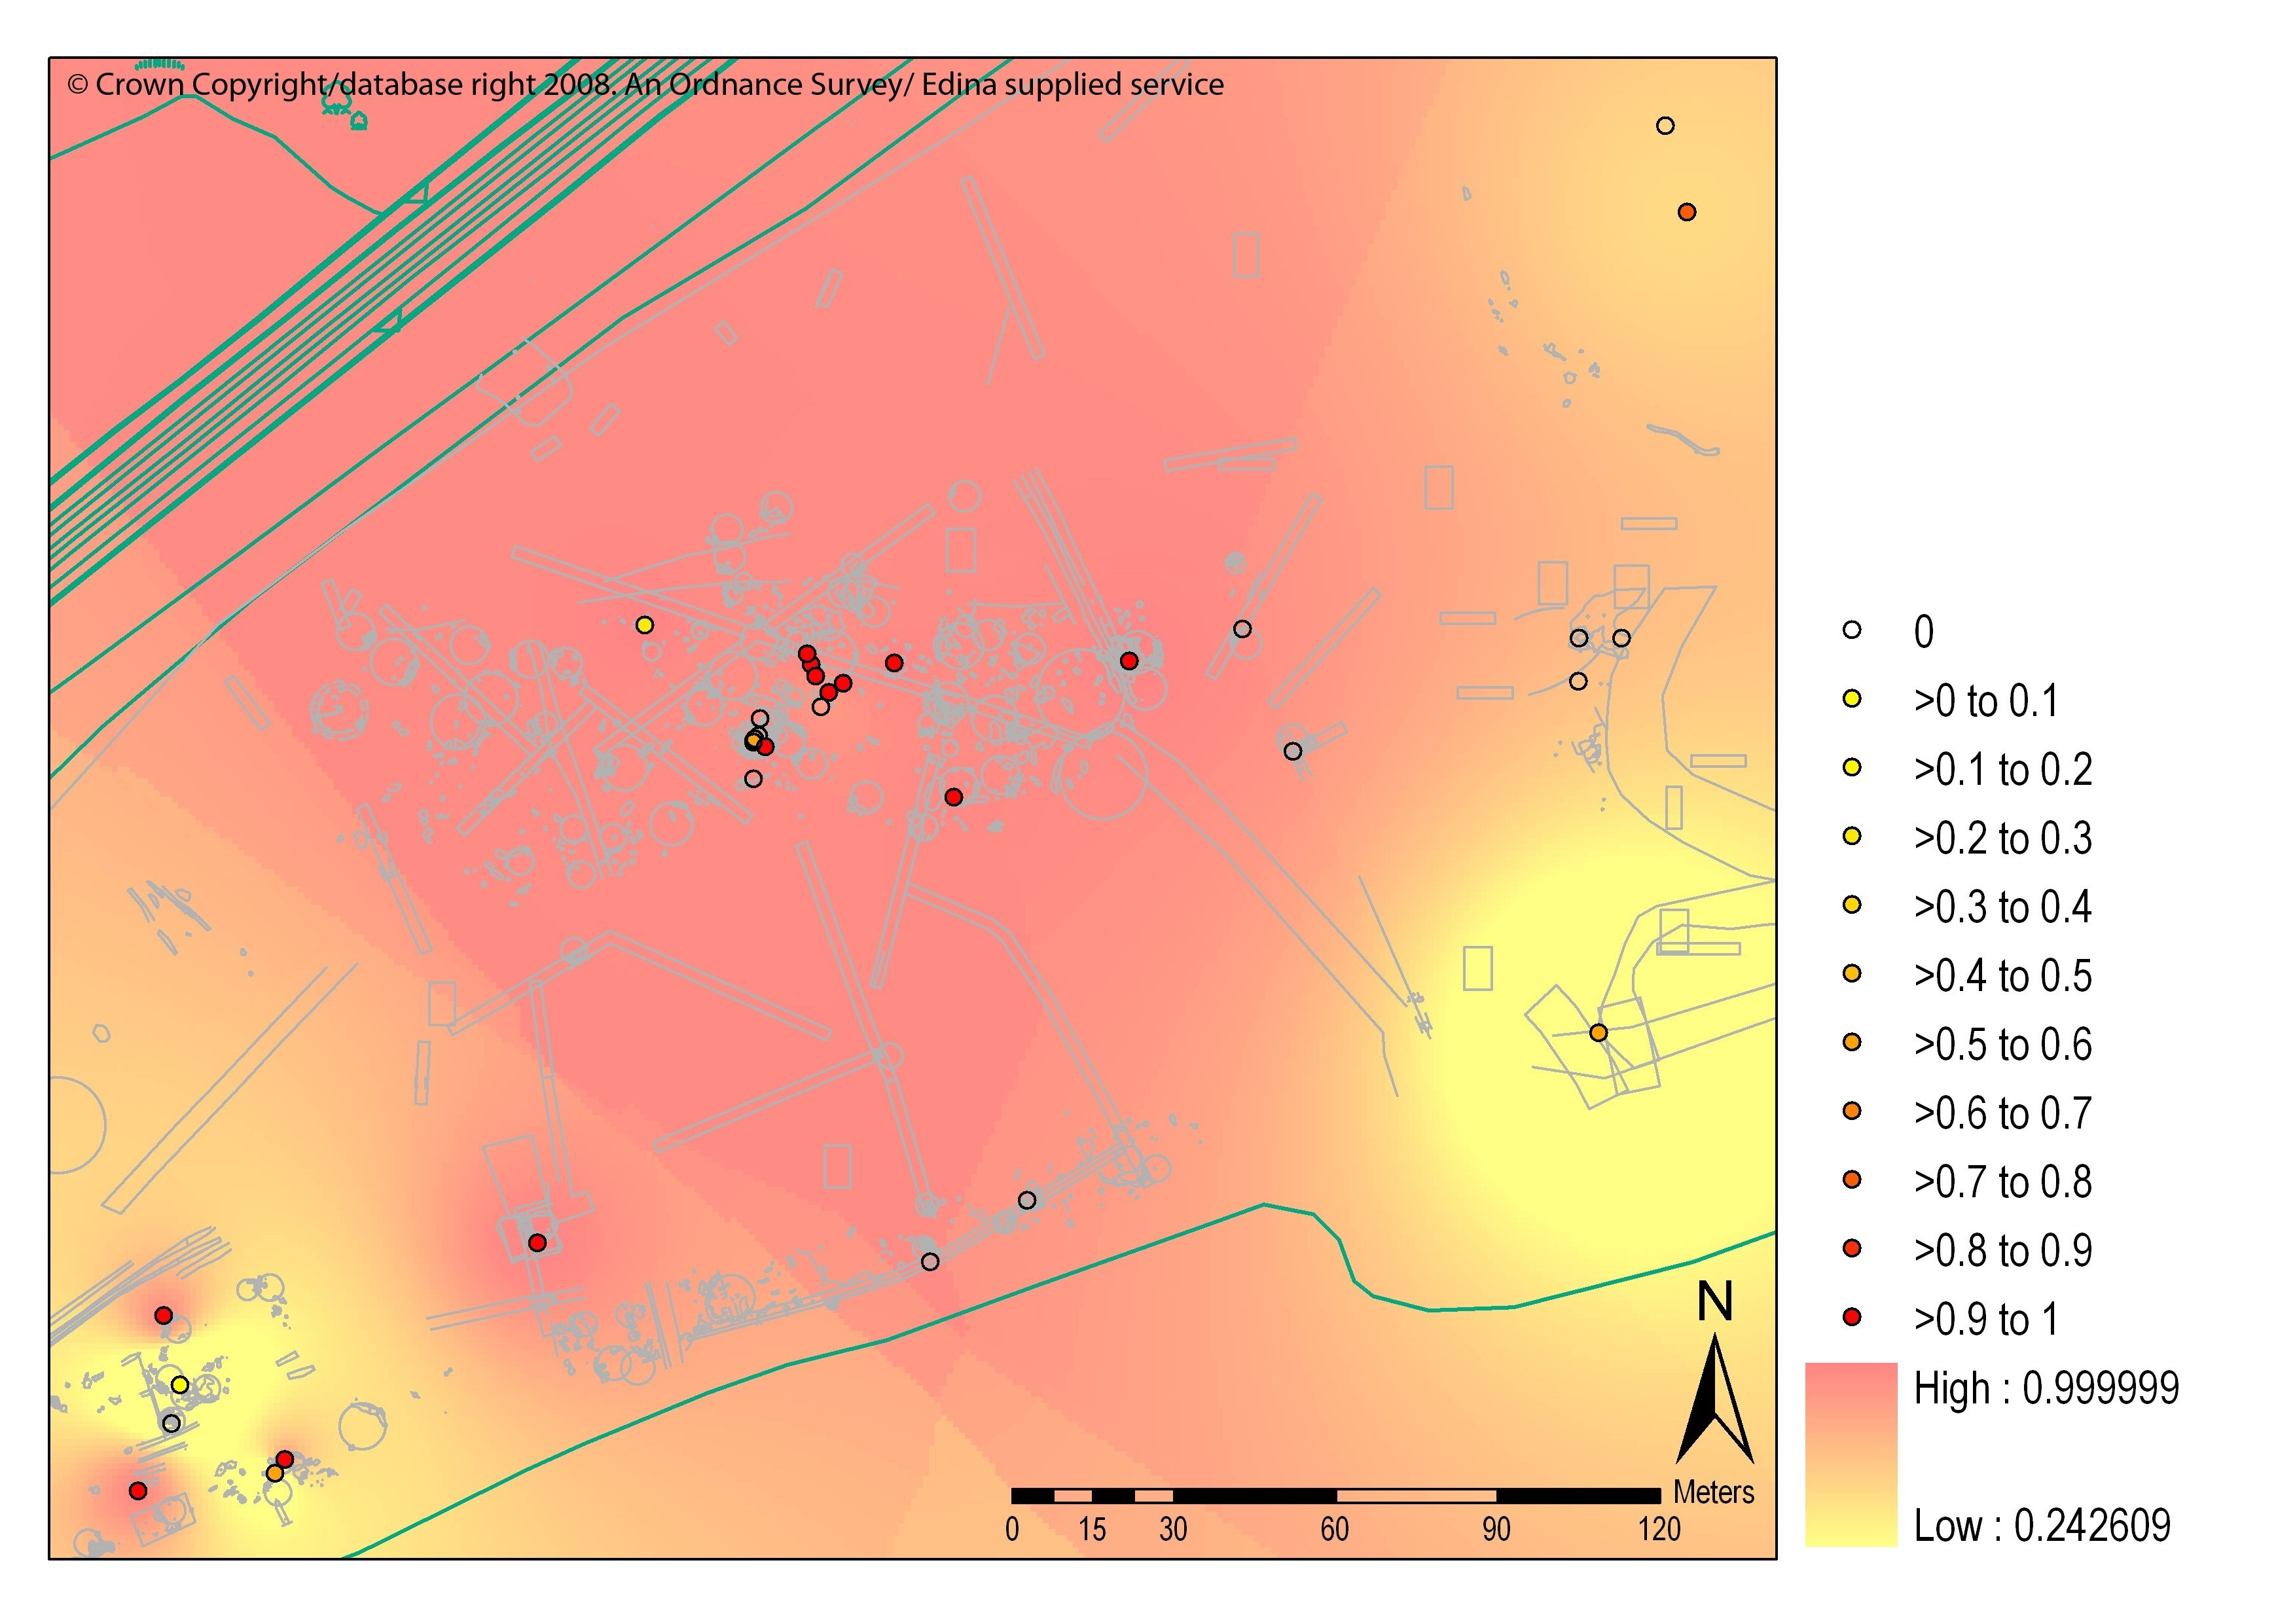
\includegraphics[width=0.9\textwidth,height=0.9\textheight,keepaspectratio=true]{figures/green2}
  \caption{Inverse distance weighted interpolation of bayesian probabilities: 3500-3000 cal BC, from \cite{Green:2008fk}}
  \label{fig:green2}
\end{figure}

Green's second use of interpolation, an inter-site case study, is effectively demonstrating the improvements in interpolating using his T-GIS, see figure~\ref{fig:green3} for an example output. However this still suffers from the problems with interpolations, including those that Green himself detailed. His crucial enhancement is that rather than points being assigned to specific phases, they instead have a probability function, which is used to determine the likelihood each point falls within a phase. This means that the data points can influence multiple phases and that in this case coarse ware pottery, which has more vague time spans, can be included alongside fine wares. He claims his method is an improvement on other similar approaches, such as aoristic analysis or p-use values, but provides no explanation or results to back this. In fact, the differences between his approach and an aoristic one are limited, with the time spans for each point in the interpolation split uniformly between phases just as in \citet[35]{Johnson:2004fk}. The difference is what happens next, Johnson sums the probabilities for each period to show how use changes over time (this description is truncated for brevity) in comparison to Green who interpolates for each phase, to show how such probabilities of use change spatially. Green claims that, unlike aoristic analysis, his method is ``not swamped by undiagnostic material'' \citep[224]{Green:2008fk} but does not back this up in any way. I would argue his approach is very similar to aoristic analysis, and his T-GIS could probably provide a convenient platform for performing it due to its discrete phase-based temporal model, and ability to split a probabilistic date into such phases. 

\begin{figure}
\centering
	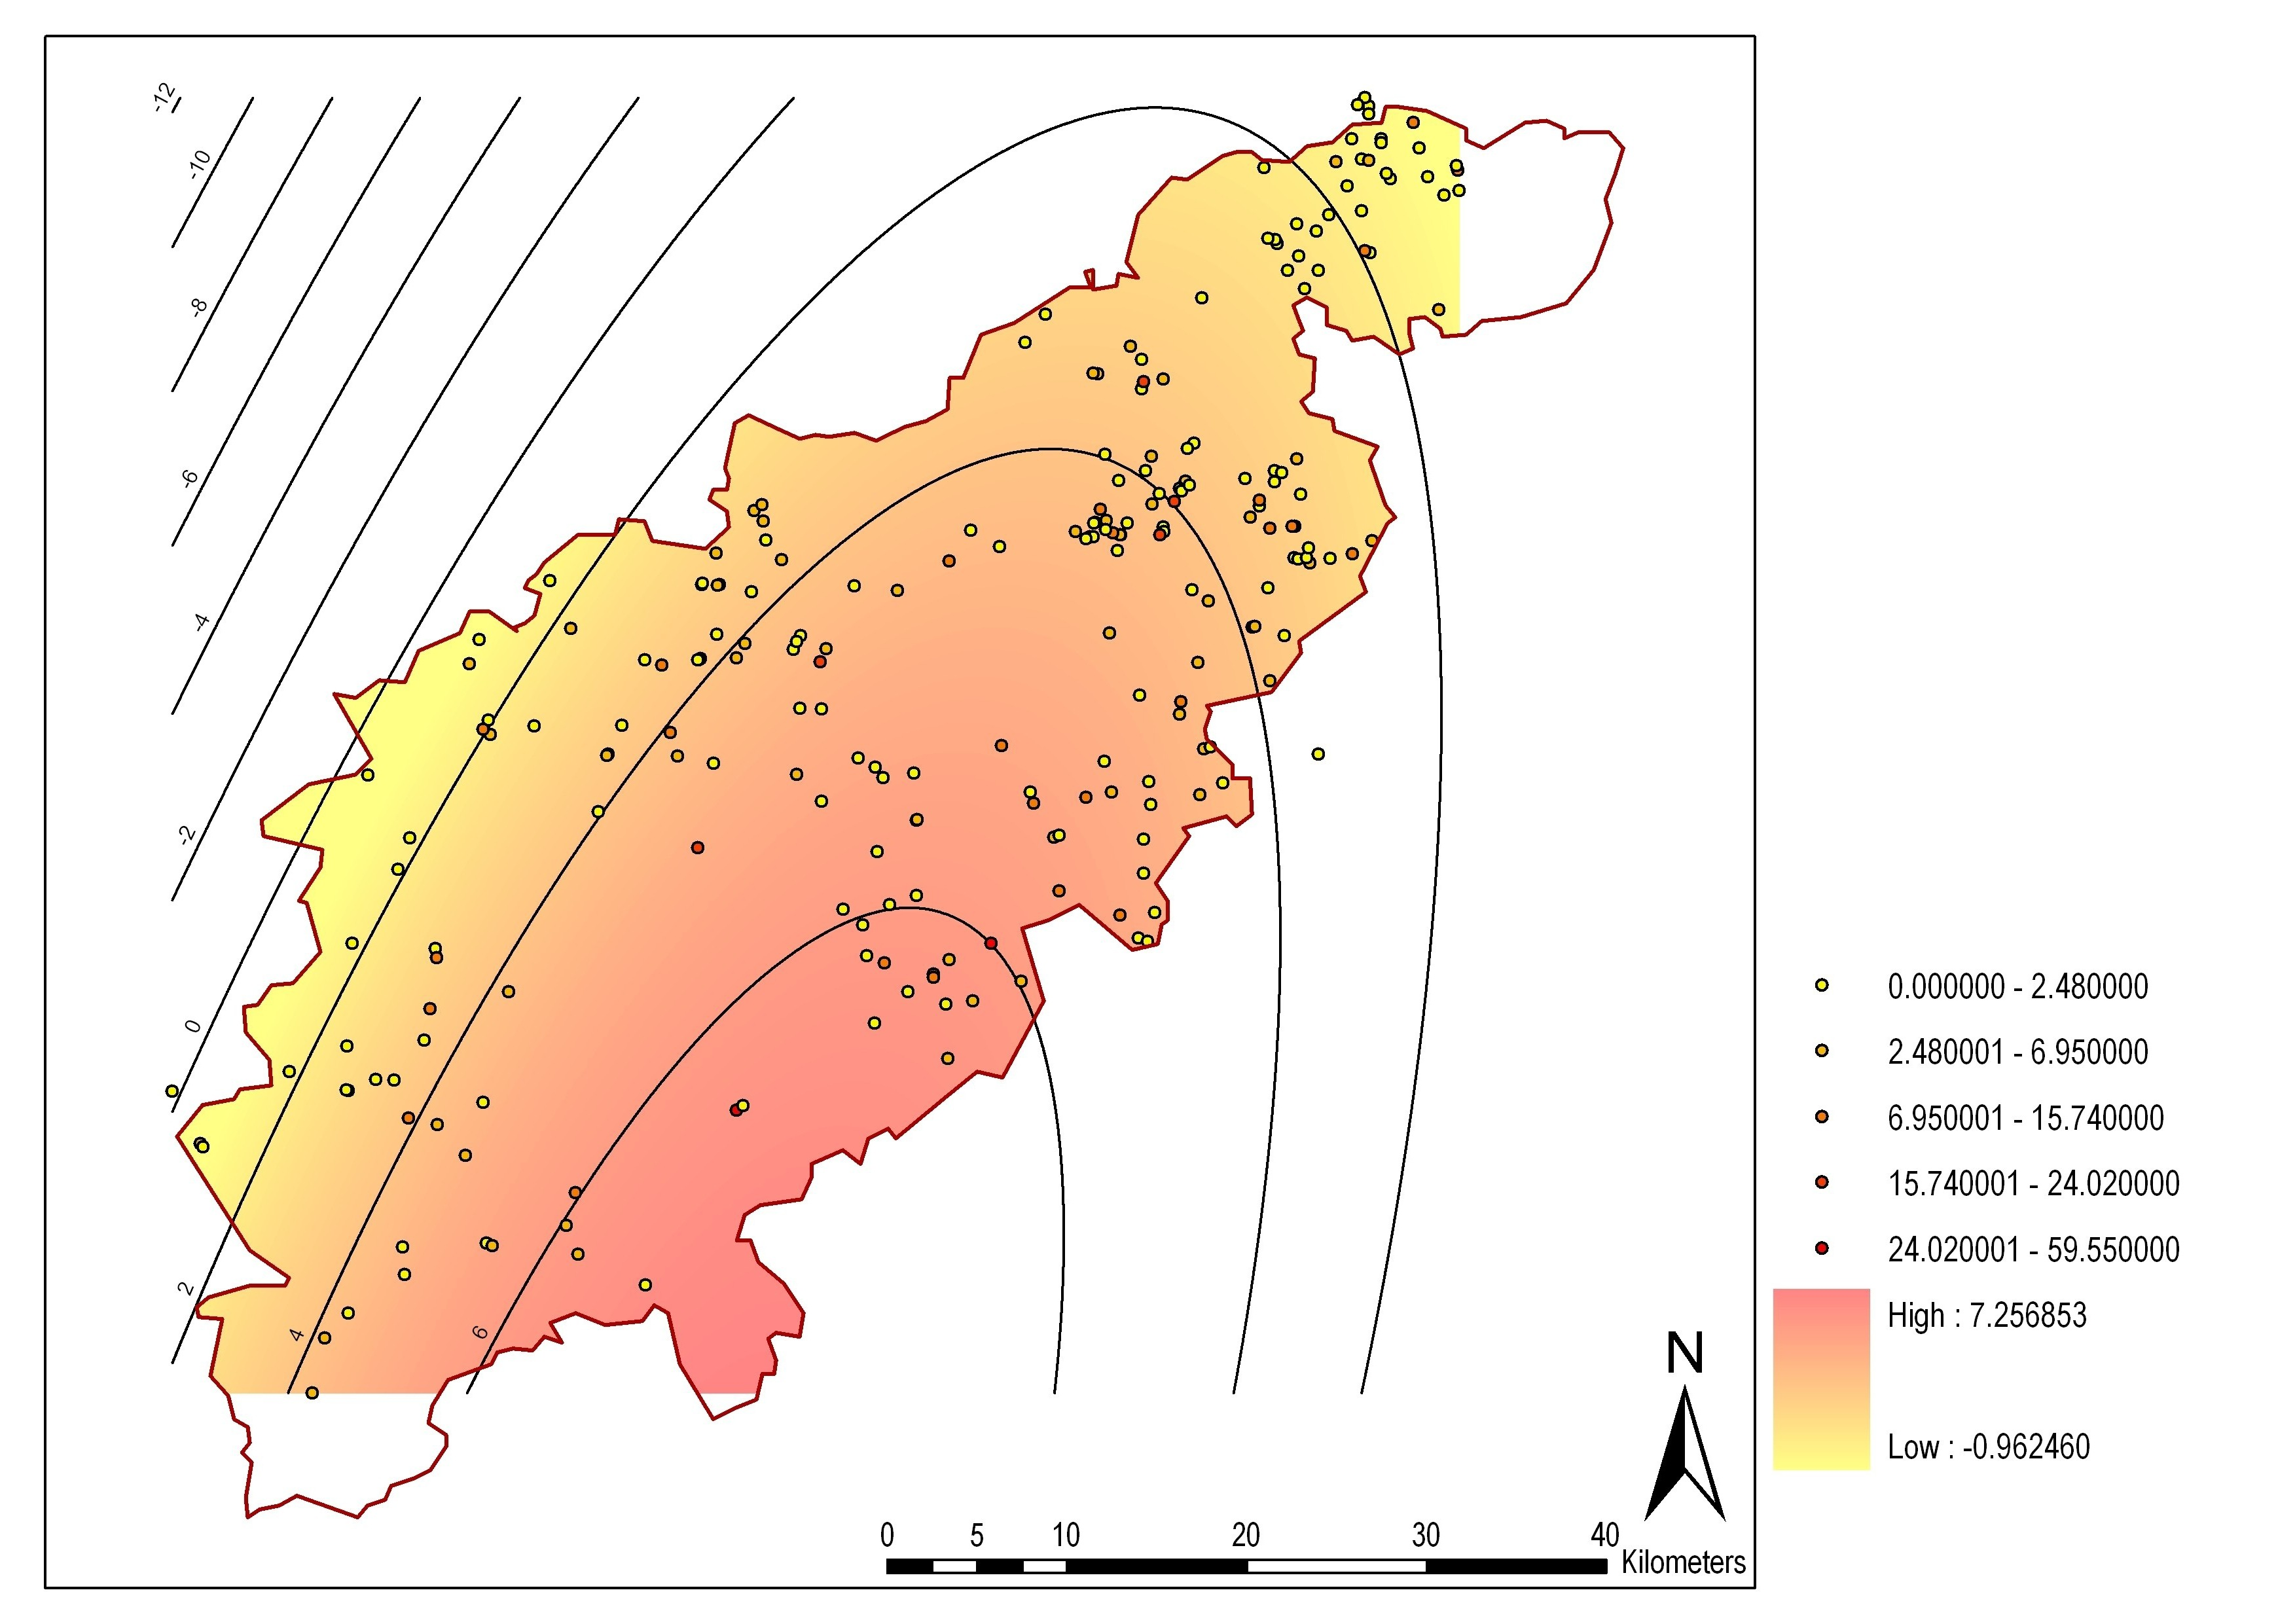
\includegraphics[width=0.9\textwidth,height=0.9\textheight,keepaspectratio=true]{figures/green3}
  \caption{Trend surface for Early phase (100 BC to AD 50) based upon TGIS probability output
normalised by sherd count. The point data layer shows the summed TGIS output, coloured from
yellow to red according to the parameter of summed probability multiplied by sherd count. The
trend surface is also shown in yellow to red, varying from low values to high, from \cite{Green:2008fk}}
  \label{fig:green3}
\end{figure}

Moving now to the tradition of spatio-temporal analysis outside of T-GIS, Johnson's introduction of aoristic analysis to archaeology \citep{Johnson:2004fk} has been noted. Specifically, as a method of analysing temporal data based on time-slices, rather than arbitrary periods and using probabilistic methods to account for the inherent uncertainty in most archaeological dates. The `aoristic weights' are ``often used as a proxy for evaluating change in the total counts of events across time'' \citep[448]{Crema2012}. Johnson made some changes to the method, which he called standardised aoristic weights, that correct for fact that modern artefacts could be assigned to individual phases with a probability close to one, whereas Palaeolithic artefacts would be assigned across so many phases they might only contribute 0.1 to each. \citet{Crema20101118} describe the peaks in aoristic weights as ``clusters of `high' knowledge'' \citep[1121]{Crema20101118} although, as they could be the result of a large quantity of data points of low probability values, the accuracy of that statement depends on what is meant by the term `high' knowledge. Does one actually know anything more about such periods than those which have a small number of data points with higher probability values? \citet{Crema2012,Crema20101118} augmented the ``vanilla'' aoristic approach by using the aoristic weights to determine whether to include a data point in a monte-carlo simulation, with \citet{Baxter2016120} providing more formalism to model generation. The resulting hypothetical spatio-temporal patterns were then analysed to determine if there was clustering in the pattern, \citep[1122]{Crema20101118} or if there was a significant change in the value of the modelled variable \citep[452]{Crema2012}. The clustering was categorised into three categories, these outcomes were then turned into percentages, and finally the probability for each cluster category. The concern with this approach is the cumulating uncertainty, starting with the original dating, then the aoristic value, next the simulations, which must include a degree of uncertainty and finally the reported probability of clustering. While there are a large number of simulations, they are only as valid as the aoristic analysis and original dating. There is also no probability attached to each simulation, some will be more likely if they include many features which have a greater likelihood of occurring in that time step. The resulting probability of clustering is based on the number of such simulations that have a clustered pattern of data.

 \citet{Crema2012} attempted to factor in the randomness derived from the monte-carlo simulation, by also computing a simulation where all of the events span the whole time frame (still with a uniform distribution) \citep[452]{Crema2012}. The rates of changes from this simulation are used as baseline of randomness from the simulation and only changes that are greater than this baseline are treated as a pattern in the underlying data. While this is a reasonable precaution, it raises two issues. Firstly, an acceptance by \citet{Crema2012} that the monte-carlo simulation will create additional uncertainty in the output and secondly by filtering it out in such a way only large changes were displayed, this meant they had to conclude that ``the outcome of the analysis did not point out radically new trends'' \citep[458]{Crema2012}. At best, their method was only able to suggest the potential for increases or decreases, but was not able to suggest numbers with any confidence, or even with an attached probability. This means it cannot really suggest the magnitude of increase or decrease and it is only capable of reliably reporting on larger changes. Surely the aim should be to refine data (as in bayesian modelling) not to make it more vague?

Fundamentally the problem with this method stems from its premise to ``identify novel patterns that are otherwise undetectable with traditional methods due to their coarse chronological resolution'' \citep[1125]{Crema20101118}. By trying to tease additional details out of probabilistic data, which only exist as an uncertainty, there is a real risk of treating the probabilities as pragmatic certainties when in fact they may not be so at all. It is perhaps more important to work with the probabilities, rather than trying to find information, which might not be there and is just a mathematical mirage.

The combined aoristic and monte-carlo approach as demonstrated by \citet{Crema20101118,Crema2012} has been taken up by other authors and adapted, for other spatio-temporal analysis. For example, land use has been investigated using this approach by \citet{ARCM:ARCM12182}. In this case, the temporal uncertainty was dealt with via simulation, during each simulation each archaeological feature was given a random date in its life span \citet[6]{ARCM:ARCM12182} - effectively modelling a uniform probability. Likelihood of an area being in use was the proportion of simulation runs that showed the area in use during a specific time slot, these were then interpolated to create iso lines of occupancy likelihood across the area being studied. In addition, categories were applied to each site, so that probabilities for use can be filtered by category, contour maps were created by category as well.

Other novel spatio-temporal methods have attempted to analyse changes in land use patterns by taking locations that are in use at a known time and then interpolating with that data to create contours of use, where the contours mark the probability of an area being in use at a specified time. This is the approach taken by \citet{ARCM:ARCM578} who use a kernel density estimate of spatial location to account for the fact that much archaeological material remains undiscovered \citep[1014]{ARCM:ARCM578} and a different kernel density estimate approach for the temporal data, which also averages out radiocarbon determinations as sites may have different numbers of radiocarbon dates \citep[1019]{ARCM:ARCM578}. Unusually, this approach formally deals with both temporal and spatial uncertainty in archaeological data to provide a model for showing changing land use in an area. The results are a series of contour diagrams, taken at 1000-year intervals. These diagrams show the effective spatial clusters created by the kernel density estimate, for each time slice. While the use of spatio-temporal probabilities is of significant value, creating spatial clusters in this way is of limited use. Take, for example, figure~\ref{fig:kde} which contains six active sites, in three groups, of two sites. Two sites form the basis for two of the clusters with another two sites broadly in between and one is pulled into the outer contours of one of the clusters. The diagram does not indicate what basis the central two sites do not form their own cluster, it is perhaps down to the weight of the temporal evidence. Alternatively, it may be an artefact of the algorithm, attempting to create the smallest number of clusters. In addition, the resulting land use values do not take into account the landscape over which they are draped (apart from excluding the sea) so areas of the landscape that may have geographical reasons for making them unusable (such as rivers, cliffs, etc) are smoothed out by the algorithm. There is little discussion or investigation of potential causes for areas to be used more during certain periods and also little discussion of the reasons or processes for that use to change, perhaps this is left for further work. 

\begin{figure}
\centering
	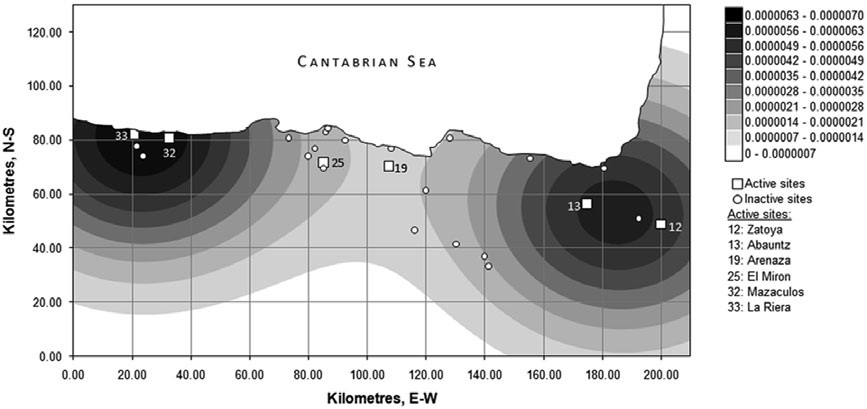
\includegraphics[width=0.9\textwidth,height=0.9\textheight,keepaspectratio=true]{figures/kde-plot}
  \caption{A bivariate KDE plot. Contour lines divide the
complete distribution into ten equally sized divisions per figure to indicate predicted density of population. Reproduced from \citet[1024]{ARCM:ARCM578}}
  \label{fig:kde}
\end{figure}

\citet{Demjn2016100} note that all of these approaches to spatio-temporal analysis are about quantifying past human activity, which is used to suggest intensity of activity, or by some authors as a direct proxy to population size \citep[100]{Demjn2016100}. Instead, \citet{Demjn2016100} set out to prove the link that ``variations in spatio-temporal distribution of archaeological settlement evidence mirror changes of settlement patterns'' \citep[102]{Demjn2016100}. Unlike previous work they first tested the mathematical model used to create the spatio-temporal distribution against simulated data to prove its validity, determine for what levels of site resolution it was valid, and compare to other methods, such as those by \citet{ARCM:ARCM578} and summed radiocarbon techniques. Their method relies on several unstated assumptions:
\begin{enumerate}
\item The mathematical model is valid;
\item Chosen model parameters are meaningful;
\item Variable feature visibility due to cultural behaviour has been ruled out.
\end{enumerate}

Point one is obvious, however the mathematical model presented by \citet{Demjn2016100} uses formulae that assumes the site and the archaeological activity are cylindrical in nature, such as that for calculating the intersection of two disks \citep[103]{Demjn2016100}. There is also the inclusion in the formula for the expected half-life of a site, although, nothing to suggest that archaeological sites have such a value in practice. Finally, this model has many similarities to the p-use representation of spatio-temporal data by \citet{Lock:1997vn} although they presented no formal method for computing activity. For point two, the model parameters for expected site radius and duration are somewhat arbitrary, with the site radius chosen as ``the average area of 20 ha (an estimation of an average prehistoric village and its immediate economic/agricultural hinterland'' \citep[104]{Demjn2016100}. Clearly this is only valid in certain locations at specific times, and would require replacing to use the model in other areas (or at least justification for retaining the same value) this is not a problem per se, but it does appear to be a very broad average which surely must hide significant variation across space and time. Point three is included by the authors themselves, ``if we are able to rule out effects of altered visibility due to cultural behaviour, the detected fluctuations can be interpreted as variations in actual settlement patterns'' \citep[106]{Demjn2016100} this is a big if, and is not addressed by the authors. It remains to be proved that it is possible to rule out these effects and until then, the usefulness of this approach is debatable.

Spatio-temporal analytical methods are varied, so far relatively under used and certainly under evaluated. The notion of additional information being present in radiocarbon distributions appears to have been adopted from more temporal studies, with the methods used to extract this hidden information becoming increasingly involved. Clearly a critical evaluation of methods is required before their results can be readily adopted, as has happened with bayesian modelling. This evaluation has taken a broad, rather than a forensic look at a range of methods that might be helpful in answering the kind of questions examined in the last chapter. Many methods have either methodological issues or complexities with their application. Fundamentally, as \citet{Torfing2015203} noted it is important to consider how the data we have relate to the questions we wish to answer and to pick an appropriate method based on this. 

\section{Alternative Approaches to Spatio-temporal Analysis}
This chapter has reviewed a wide range of quantitative analysis, starting with a brief review of spatial methods, a detailed examination of the two most prominent temporal techniques, followed by a review of the limited spatio-temporal methods available. The observation on spatio-temporal techniques by \citet{Demjn2016100} that most, if not all current methods focus on quantifying the intensity of past human activity is crucial, such methods are likely to easily fall foul of the issues identified by \citet{Torfing2015193}. Specifically any attempt at analysing activity must make assumptions to do with how archaeological material relates to ``activity'' (or population) it must then account for changes to the archaeological material post deposition and how archaeological recovery might affect patterns in the data. To dismiss such a line of research in its entirety at this stage would clearly be an over reaction, but surely there are also plenty of opportunities for a more contextualised school of spatio-temporal analysis. Such a school could be based around taking existing temporal methodologies and either extending them or performing additional spatial analysis. A key benefit of this approach is the ability to adopt methods for working with different scales of archaeological data, as the opportunity presented by a site wide data set is clearly very different from that presented by a continental scale data set. In order to achieve the aims of this thesis, of re-combining spatial and temporal data for unified analysis and of pushing forward the boundaries of such study it will be essential to explore the possibility of spatio-temporal analysis using such varied data sets.

In order to effectively work with and perform analytical procedures on such data sets it is likely that specialist software will be required. The subject of Temporal GIS is clearly a potential source for such tools, a thorough examination of the development and use of these tools will be required to understand how they can be effectively utilised to extend existing temporal techniques to include spatial data.